%% future_work.tex
Deep learning is far from being a system with human-like intelligence. Consequently, there is a massive amount of work to be done in the future to get closer to this ultimate goal (while the goal should still be to build a system that supports humans and not behaves like one). However, the implementations presented in this thesis are far from such a system. Consequently, a conclusion is drawn, and the next steps are proposed for the models presented in this thesis, but a long-term vision is presented as well. Specifically, some insights are given to the neuroscientific concept that seems very promising in section \secref{future_neuro_concepts}, and future work is described for horizontal self-organisation in \secref{future_hso} as well as for vertical self-organisation in \secref{future_vso}. Afterwards, in \secref{future_3_stage}, a new model is presented on a very abstract level, which could work better intuitively, but a concrete implementation is unclear. In \secref{useful_representations}, the usefulness of representations is discussed. In the last \secref{cognition_reasoning}, the author gives a personal opinion about the future of AI, which is not supported by scientific arguments but might be interesting for (motivated) readers.



\section{Neuroscientific Concepts}\seclbl{future_neuro_concepts}
In \chref{neuro_concepts}, several concepts from neuroscience are identified that are believed to be fundamental for biological intelligence. However, since the discrepancy between biological and artificial models is large, it is difficult to incorporate these biological concepts into a computer system. This thesis makes concrete suggestions on how such concepts can be implemented. Implementing these concepts in the form of horizontal and vertical self-organisation demonstrates that these ideas can facilitate the learning process. The evaluation of the suitability of neuroscientific concepts was very iterative: many concepts were tested but discarded in the course of the work because they did not add enough value to existing systems. For example, much time was spent on sparsifying activations over several time steps as it is done in the human brain. However, it was found that the sparsification of representations over several time steps has no advantage without additional system dynamics. This could be because the data is static and already contains all the information. Therefore, the result is the same if the sparsification is done in one time step.

The most promising concepts identified in this work for improving deep learning systems are self-organisation, net fragments, sparsity\sidenote{but not over time}, lateral connections, continuous input, and embodiment. For each of these mechanisms, a concept for implementation is proposed, except for continuous input and embodiment. However, these proposals are the author's interpretation and are only one of many possible solutions. These concepts can also be interpreted differently, and an alternative implementation could also lead to promising results. Furthermore, exploring continuous input and embodiment in future work could help to build more intelligent systems. 


\section{Implemented Models}\seclbl{future_so}
The concepts from neuroscience are implemented in two specific ways, these are called horizontal and vertical self-organisation. It is important to note that the implementation of \emph{neuroscientific concepts} is the main focus of this thesis and not to push scores like accuracy on benchmarks. In general, a comparison with end-to-end backpropagation of error is not appropriate in this field: Backpropagation has been optimised for over 30 years by many institutes and even more researchers, and therefore alternative learning concepts cannot be expected to outperform backpropagation of error instantly. Thus, backpropagation of error is not considered an appropriate baseline.

Rather, the proposed implementations showcase interesting neuroscientific concepts. However, the implementation has not yet been optimised and incorporated in big networks that might perform on the level of existing systems. Rather, these implementations are to be understood as a basis for future work (c.f. \secref{future_3_stage}, \secref*{useful_representations} and \secref*{cognition_reasoning}) that improves AI in the long-term.


\subsection{Horizontal Self-Organisation}\seclbl{future_hso}
TODO: this section is not yet complete as many experiments are still ongoing...

The proposed horizontal self-organisation approach uses a novel proxy objective function. Models based on proxy objective functions are biologically more plausible and a hot research topic (c.f. \secref{alt_train_algo}). Recently, many algorithms have been proposed, such as the forward-forward algorithm \sidecite{ff_algo}, which have caused a stir in the community by challenging the classical backpropagation of error as an optimisation algorithm. However, despite the fact that algorithms using proxy objective functions are biologically more plausible, these algorithms do not provide many benefits yet. Models trained with backpropagation of error are still superior, especially on well-known tasks such as classification. One of the author's hope was that such algorithms have other advantages, such as better robustness. However, evaluating the models presented in this work and other models, such as the forward-forward algorithm, has crushed this initial belief: No model that uses proxy objective function achieved better results on the corrupted MNIST-C dataset than end-to-end backpropagation of error.

For classification, a sample is compared to the average activation of each class. This average activation can be understood as an object prototype within a world model. Thus, it is compared to which prototype a sample fits best. The problem is that a single object prototype is not sufficient. As an example, \figref{digit_4_versions} shows different versions of the digit $4$ that can be found in the MNIST dataset. This shows that a digit can be written in different ways\sidenote{this applies to all kinds of datasets: Most objects can have various visual characteristics (size, colour, shape) or look different from different viewpoints}.
Consequently, the digits and, thus, the activations look different for samples from the same class, and the use of more than one prototype per class seems helpful. Thus, instead of calculating the average activation per class, it could help to divide the activations per class into representative groups using a hierarchical clustering algorithm and to calculate the average activation (i.e. the cluster centre) per group. By doing so, multiple representative prototypes per class are obtained, and the prediction could become a lot more accurate.

\begin{figure}[h]
    \centering
    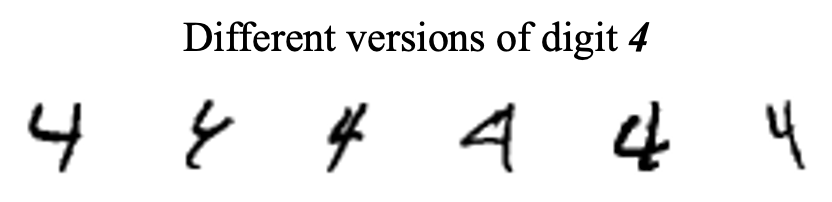
\includegraphics[width=0.49\textwidth]{digit_4_versions}
    \caption[Different versions of the digit ``$4$'' in the MNIST dataset]{Different versions of the digit ``$4$'' in the MNIST dataset.}
    \figlbl{digit_4_versions}
\end{figure}


The generated representations have so far only been examined for classification. However, since the objective function does not explicitly optimise the model for classification, it would be interesting to investigate what other information is contained in the representations. Furthermore, the representations are currently generated with a supervised approach since the labels are used in the loss function. However, the use of labels is generally not desirable because the manual creation of labels is labour-intensive. On the other hand, an unsupervised (or self-supervised) approach extracts features without labels. Moreover, it is known that the brain also learns unsupervised to a large extent and is thus biologically more plausible.
Thus, the implementation of a loss function that does not rely on labels would be beneficial. Furthermore, the model should be tested on other datasets than MNIST to evaluate how well it can scale.




\subsection{Vertical Self-Organisation}\seclbl{future_vso}
TODO: this section is incomplete as many experiments are ongoing...

Vertical self-organisation splits the input image into multiple patches and processes each patch with an independent model.
Similar to horizontal self-organisation (c.f. \secref{future_hso}), the prediction accuracy could be improved by using more prototypes per class, as digits of the same class can look different. In the case of vertical self-organisation, the $\boldsymbol{\mu}$ values per VAE should be clustered hierarchically to obtain groups of similar-looking digits per class. Afterwards, the average value per group can be calculated to obtain more prototypes per class.

An essential concept in the human brain is the prevention of early commitment\sidecite{Marr_2010} (c.f. \secref{future_3_stage}), i.e. that a single entity such as a network layer not commits to something and then persists. Typical CNN architectures for classification have this problem by design, as they combine low-level features into higher-level features. Low-level features are detected locally; thus, it is already determined which feature is within the image before global information is considered. The proposed architecture for vertical self-organisation reduces this problem by creating representations of image patches. The patches are so small that they contain only enough information to build low-level features. For example, the representations from a single VAE cannot be clearly assigned to a class and thus do not contain enough information to commit to an object. Therefore, the VAEs can be considered low-level feature extractors, such as the first layer of a convolutional network. To create higher-level features, communication with neighbouring VAEs (i.e. when looking at the big picture) is needed. Each VAE extracts low-level features (local view) and communicates with other VAEs (global view) to determine their representation. Therefore, this architecture is less susceptible to the early commitment problem than typical end-to-end trained neural networks.
Furthermore, the representations are learned unsupervised. For classification, the labels are fed into the network \emph{after} training in order to compute average class representations. Thus, no class representation but an image representation is learned during training. This further reduces the problem of individual VAEs committing to a class.

In future work, this effect should even be intensified by further reducing the size of the patches and using more VAEs. It can be assumed that with $16$ VAEs ($4\times4$), the field of view is so restricted that each VAE can only produce very poor representations, and these can only be randomly assigned to a class. With more VAEs, communication can also be restricted locally: With $2\times2$ VAEs, each VAE automatically receives information about the entire image when communicating with its neighbours. With $4\times4$ VAEs, on the other hand, it is possible to have each VAE communicate only with its immediate neighbours. In this case, global image information must be propagated over several time steps from one VAE to the next.

Future work should also address a key problem of this architecture: Currently, this concept only works with images in which the objects always appear at approximately the same place in the image. This can be remedied if the VAEs are applied at different places in the image, similar to a kernel in a convolutional layer. In this case, however, the same VAE sees all image data, meaning that it implicitly receives local and global image information. This could reduce the independence of each VAE. Consequently, it should be investigated how this architecture can become translation invariant in a similar way as CNNs.


\section{3-Staged Model}\seclbl{future_3_stage}
Christoph von der Malsburg, co-supervisor of this thesis and one of the authors of the ``Theory of Natural Intelligence'' paper\sidenote{the work that served as \emph{the} source of inspiration of this thesis} \sidecite{von_der_Malsburg_Stadelmann_Grewe_2022}, is one of the pioneers of the theory of self-organisation of ordered fibre connections in the visual system \sidecite{Wolfrum_Wolff_Lücke_vonderMalsburg_2008, Willshaw_VonDerMalsburg_1979, wiskott1996face, Fernandes_vonderMalsburg_2015}. His theory is based on a $3$-staged model. Currently, the author and supervisors of this thesis are working on writing down this model and relating it to current deep learning architectures. Writing it down should enable non-neuroscientists to understand these exciting concepts better and to relate them to the context of deep learning. The resulting (hopefully publishable) paper will not be included as part of this Master's thesis, as it was not written by the author alone. Nevertheless, it explains exciting concepts that are promising for future research and highly relevant to this thesis.

Von der Malsburg's theory refers to an image perception model with three stages S$1$-S$3$, and projection fibres between these stages.
The stage S$1$ refers to the first stage, which is responsible for the extraction of features from images. In this stage, one fundamental principle is to avoid the ``fallacy of early commitment''. \sidecite{Marr_2010}.
The idea is that local decisions should only be taken if plausible in the light of high-level features, while high-level features can only be defined based on low-level patterns.
The brain can handle this very well, as the Gestalt psychology shows\sidenote{Gestalt psychology is about intelligent beings perceiving entire patterns, not individual components}. \sidecite{kohler1929gestalt}.
Modern deep learning networks cannot deal with this and often recognise patterns in the first layers, committing to something specific that is something else in the light of the big picture. The core mechanism in the human brain to deal with this is, according to von der Malsburg, a mechanism based on lateral connections between neurons that are spatially close to each other. Initially, many neurons are activated by the retina's impulses. However, these neurons are immediately turned off if they do not have sufficient lateral support from neighbouring neurons. The lateral connections are thus there to support each other to remain active. This not only has the effect of ``mutually confirming each other'' but also helps to form higher-level features from low-level patterns: There are oscillations in the brain that also influence the number of active neurons. In other words, more neurons are constantly activated and then fewer again. Only those with the greatest local support remain if the number of active neurons is reduced. Thus, many neurons are deactivated in a short time. With each reduction in the number of active neurons, higher-level features are selected by supporting them (so-called net fragments) and remain.
Since these pixel groups keep each other active, neurons that represent insignificant features are continually switched off.

The lateral support, however, is limited to local patterns, i.e. the lateral support in S$1$ is not sufficient to recognise whole objects or scenes, but only parts of them. In stage S$2$, however, these features are mapped to whole objects. These object representations in S$2$ are independent of transformation and position. Projection fibres do the mapping of several low-level features to a concrete object. These implicitly remove transformations and position information from the features and assemble them into objects. Projection fibres can be interpreted as a kind of graph that combines features hierarchically, ignoring local distortions to create transformation-independent object detection. Stage S$3$, on the other hand, stores very abstract prototypes of such objects, and by matching S$2$ and S$3$, the captured object instances can finally be d with the brain's memory.

The described model contains exciting concepts. Especially the prevention of early commitment and dynamic fibres seem very promising. However, a concrete implementation that works for complex images like natural photos has yet to be implemented, despite a lot of effort in research. There is potential in using the recently popularised graph networks as projection fibres and thus learning the projections without relying on restricted mathematical models. For example, VAE or VQ-VAE, as in vertical self-organisation, could be used as feature extractors. The advantage of these autoencoder types is that they can extract local patterns and describe them as vectors in a ``meaningful'' latent space, i.e. similar vectors lie closer together in the latent space or, in the case of VQ-VAEs, are even discrete values. This facilitates the statistical learning and mapping of similar embedding vectors together. Vertical self-organisation (c.f. \secref{future_vso}) is considered an important preliminary work to implement such a system. In contrast to vertical self-organisation, autoencoders could be applied at any image position to obtain continuous pixel representations from the same latent space. The autoencoders can thus be used as feature extractors to extract good representations of small image patches. Afterwards, graph neural networks (GNNs) could be used to combine the embedding vectors into higher-level features. GNNs have already been used for image classification in recent years, mainly by identifying super-pixels and connecting them by graphs to recognise object structures \sidecite{Long_yan_chen_2021}.  One problem with GNNs is that they are often flat, i.e. many nodes lie on the same plane. This does not comply with the model of projection fibres, which must be highly hierarchical due to the large number of possible pattern combinations. A remedy to this issue could be using differential pooling \sidecite{10.5555/3327345.3327389, Vasudevan_Bassenne_Islam_Xing_2023}.

However, the goal is not to identify objects with graph structures. Instead, the graph should be able to match objects from images with abstract prototypes. In this way, the network should learn to ignore slight transformations and rotations. For example, GNNs for object recognition could be combined with graph matching networks \sidecite{li2019graph, Xu_Nikolentzos_Vazirgiannis_Boström_2022} and thus might be used to match objects locally and globally despite slight transformations. This matching would correspond to projection fibres from L$1$ to L$2$ and compare objects within an image with mental prototypes. However, many questions remain, such as how objects are identified in images (i.e. how to remove the background) or how the mental prototypes get into L$2$ in advance in order that they can be matched. Furthermore, one must consider iterative matching to avoid early commitment: Low-level features should not commit to an object. Therefore, low-level features have to be extracted, and only a global view of all features allows to give them meaning. Thus, the learning process might iterate between updating features locally and giving them meaning in the global context.


\section{Useful Representations}\seclbl{useful_representations}
In this thesis, models are proposed that extract representations of images.
However, the question of how useful these representations are still remains\sidenote{despite the usual ML tasks such as image classifications}.

The usefulness of representation depends on the use case: Usually, good representations should contain exactly the information that is needed\sidenote{retaining as much information as possible is often not useful as this corresponds to storing (a compressed version) of the image} (i.e. be compact), be robust, be interpolable, and be well-aligned with the real world.
For example, representations from modern deep learning systems are very useful for typical vision tasks such as classification or segmentation. In some cases, deep learning representations are even superior to humans. For example, modern deep learning systems \sidecite{DBLP:conf/bmvc/JungLO0SP22} can identify millions of faces with more than $99\%$ accuracy, which is very difficult for humans \sidenote{at least to distinguish such a large number of people}. 
However, what works poorly for deep learning systems is recognising an object as the same instance, regardless of which transformations have been applied. In general, deep learning systems cannot learn a good world model and understand transformations applied to the objects of this model.

One way to address this problem is to allow the model to interact with the world (i.e. perform actions). Interacting allows a model to learn how an action changes the view of an object. Object-independent transformation behaviours can be learned if the same actions are applied to different objects. This could allow a model to understand which views represent the same object in the world model and what kind of transformations have been applied to it.

It is known from the study of animals that both eye movements and the behavioural state influence the responses of neurons in the visual cortex \sidecite{Keller_Bonhoeffer_Hübener_2012}.
Thus, animals integrate their action (i.e., their movement) with currently incoming sensory signals to predict future sensory inputs.
The internal copy of an outflowing movement-producing signal generated by an organism's motor system is also known as efference copy.
Keurti et al. \sidecite{Keurti_Pan_Besserve_Grewe_Schölkopf_2022} argue that such efference copies are helpful to learn \emph{useful} latent representations perceived by the visual system.
They translated this idea into an AI-based system by allowing an agent to interact with the environment and to observe its state to build internal representations.
They enforce that transformations of the real world can also be applied to latent representations, i.e. that the mental objects and the real-world objects remain consistent when similar transformations are applied to them.

Giving an agent an embodiment\sidenote{in this context, an embodiment can also be virtual, i.e. allow the agent to interact with objects} to interact with the world to better understand it and to create better representations seems not only important from a neuroscientific perspective but is also in line with theories from psychology.
Piaget \sidecite{Piaget_1964} argues that perceiving an object is rather about understanding how it transforms and behaves and not creating a mental copy of it.

Such an agent can be implemented, for example, with reinforcement learning.
The training process could be explicitly modelled by predicting future states based on a given state and possible actions before the action is executed and the actual outcome is observed in the world model.
This procedure corresponds to the perception-action episode that is postulated by LeCun \sidecite{LeCun_AMI}.
He divides the process into seven steps;
(i) First, the perception system extracts a representation of the current state of the world $s[0]=P(x)$. (ii) The actor then proposes an initial sequence of actions $(a[0], ..., a[t], ... a[T])$ that the virtual world model executes. (iii) The world model, in turn, predicts a sequence of world state representations resulting from the proposed action sequence $(s[1], ..., s[t], ... s[T])$. (iv) A cost model estimates the total costs for each state sequence as a sum over time steps $F(x)=\sum_{t=1}^{T}C(s[t])$. (v) Based on multiple cost predictions, the actor proposes the action sequence with the lowest costs. (vi) The actor executes one or a few actions (and not the entire action sequence), and the entire process is repeated. (vii) Additionally, every action, the states and associated costs are stored in a short-term memory that can be used to optimise the system.

Overall, it seems very important that a model does not receive a sequence of unrelated images and their labels as input, as in typical classification tasks. Instead, the agent should receive a continuous stream of related input images and information about their transformation. In this way, transformations can be observed and consciously learned, which is fundamental to understanding visual scenes.

\section{Cognition and Reasoning}\seclbl{cognition_reasoning}
At the end of this thesis, I want to share my personal opinion on how deep learning systems can be improved fundamentally: Deep learning systems can extract pixel representations from images very well. I intentionally call it ``pixel''-representations and not object representations because these vectors contain information about pixel constellations which are not sufficient to describe objects but very well suited for tasks like classification or segmentation\sidenote{end-to-end backpropagation of error seems to work excellent to generate ``pixel''-representations}. According to my definition, these pixel representations are only a part of object representations. Object representations are a mental construct that contains much more information about objects than how they look. For example, object representations should contain information about how an object behaves under different transformations. In the previous two sections (c.f. \secref{future_3_stage}, \secref{useful_representations}), it is discussed how such transformations could be learned. However, there are many other parameters that make up an object, such as what abilities it has  (e.g. can it move?) and how it feels. The appearance of an object (which corresponds to the pixel representations) is thus only one dimension of a high-dimensional formula that describes an object. For example, fish and ships look completely different on a pixel-level description and have visually nothing in common. For us humans, these two objects have a clear relationship defined by their ability to swim and the typical place where they are found, namely the sea. Another example is heat: It feels hot, and in my mental world model have things like fire, the blue flame of a welding machine, and a hob, an obvious relationship. However, all these objects look completely different.
Many modern pattern extraction systems only model one-dimensional pixel representations and not multi-dimensional object representations and thus cannot build such relationships.
Extending these one-dimensional object representations (``what does the object look like'') to multi-dimensional representations might be one of the key elements to creating a system with cognition and reasoning. This allows object hierarchies to be built on multiple dimensions: Instead of just a hierarchy of objects that look similar, we also need hierarchies of objects that behave similarly, have similar capabilities, feel similar, etc.

In addition to this construction of multi-dimensional object representations, an understanding of the world's physics is also necessary. This second type of representation summarises knowledge that relates to all objects, for example, the earth's gravitational force, the fact that living beings cannot walk through solid materials such as walls, etc. The question that arises now is how such a system can be implemented. It is obvious that more than simply showing pictures and the corresponding labels is required to learn such complex relationships. At least three key elements are required:


\begin{description}
	\item[The world] in which the agent lives must allow interactions. This allows the agent to learn representations better; for example, getting visual observations together with efference copies allows an agent to understand how objects behave. Furthermore, such a world allows understanding differences and similarities between objects. It also allows the agent to define what it does not yet know and to learn these things consciously (for example, with an entropy-based loss function \sidecite{storck1995reinforcement}). Thus, continuous input is necessary. Training a model with a sequence of random and unrelated images is most likely not sufficient.
	\item[The network architecture] must enable and encourage the capture of the world structure. I think that a multi-dimensional world model is helpful for storing and relating the appearance, behaviour, transformation capabilities, abilities, etc., of each object and a second model to store general knowledge about the world. Such a model allows for a multi-dimensional relationship between objects and a better understanding of them\sidenote{in a pure vision perception model, a division into the dimensions of appearance, behaviour during transformation and physics (e.g. the object is standing on the ground) would already be a massive step forward}.% Multi dimensional world model, per object appearance, transformation behaviour, abilities, feeling, smell, ...
	\item[The learning algorithm] should consider several things to learn a good world model. A key element is that the learning algorithm decides what to learn (entropy based on the knowledge in the world model). Furthermore, curriculum learning seems promising: for a high level of intelligence, an equally complex world must be available in order to be able to learn it. However, such worlds might be so complex that the agent is overwhelmed without a step-by-step complexation of the world\sidenote{this also applies to humans: We have prior knowledge through evolution, and then our parents explain the world to us. In fact, we are not able to survive without proper support in the first years}.% continuous learning, curriculum learning % LLM -> predicten next token -> predicten objects next state
\end{description}

An intelligent system consists of several components: One very crucial component is the perception system. From today's point of view, this is the component that is best mastered, i.e. deep learning systems can capture useful patterns in high-dimensional data very well\sidenote{although there are things that need to be improved, c.f. \secref{future_3_stage}}. Around this system, a world model has to be created, which stores the understanding of the world. It is important that the agent learns to learn, i.e. finds out for itself what knowledge it lacks in the world model and acquires it from the real world. Such behaviour can be implemented by an entropy-based loss function \sidecite{storck1995reinforcement}. The second question is what knowledge is extracted from the world and stored in the world model (and thus implicitly defines what the agent learns). The knowledge stored in the world model should be multi-dimensional object information, as described in the first paragraph of this section, which provides a much richer understanding of the world than the current one-dimensional pixel representations. To get a real understanding of the world, interactions with the world and predictions of how the next state of the world looks seem to be very central\sidenote{for example, the simple task of predicting the next token of a text has led to the enormous capabilities of large language models}. A straightforward implementation is a roll-out (i.e. predict how the world looks like after applying some actions and comparing this to the real world after these actions have been applied) \sidecite{LeCun_AMI}, more advanced seem to be GFlowNetworks \sidecite{NEURIPS2021_e614f646}. After such predictions are learned, reversing this process, as in diffusion models, could be a first step towards casual reasoning. In diffusion models, one learns to map from a specific state (a concrete image) to a very general state (noise). This process is reversed, and over several steps, the model can build trajectories from noise to a sample through a combination of direct and random motions. If a similar concept is applied to the learned prediction of actions, it can be predicted which action combinations have led to the current world state.

However, all these ideas are very abstract and have emerged in the course of this work. The concretisation of these ideas could take years and, unfortunately, are out-of-scope of this thesis. However, I hope to be able to address such questions as concrete research topics soon, ideally in a similar constellation as in this Master's thesis.

